\documentclass{article}
\usepackage[french]{babel}
\usepackage[utf8]{inputenc}
\usepackage[T1]{fontenc}
\usepackage{graphicx}
\usepackage{algorithm}
\usepackage{algorithmic}
\usepackage{amsmath}
\usepackage{systeme}
\usepackage{float}
\usepackage{amssymb}
\usepackage{mathrsfs}
\usepackage{color}
\usepackage{fancyhdr}
\usepackage{pdfpages}
\usepackage{layout}
\usepackage{multicol}
\usepackage{setspace}
\usepackage{caption}
\usepackage{csvsimple}
\usepackage[table]{xcolor}
\usepackage[colorlinks=true]{hyperref}
\usepackage{tikz, tkz-tab}
\usepackage[top=2cm,bottom=2cm,left=1cm,right=1cm]{geometry}
\usepackage{amsthm}
\usepackage{algorithm}
\usepackage{algorithmic}
\usepackage{multicol}
\usepackage{textcomp} 
%%%%%%%%%%%%%%%% Lengths %%%%%%%%%%%%%%%%
\setlength{\textwidth}{18.5cm}
\setlength{\evensidemargin}{-1.0cm}
\setlength{\oddsidemargin}{-1.0cm}

%%%%%%%%%%%%%%%% Variables %%%%%%%%%%%%%%%%
\def\project{6}
\def\title{Résolution approchée d'équations différentielles et modélisation de systèmes dynamiques}
\def\group{3}
\def\team{1}
\def\manager{Raphaël Blard}
\def\secretary{Simon Triscos}
\def\others{Imad Boudroua, Mohamed Fayçal Boullit, Antoine Dudouit}
\def\R{\mathbb{R}}
\begin{document}

%%%%%%%%%%%%%%%% Header %%%%%%%%%%%%%%%%
\noindent\begin{minipage}{0.98\textwidth}
  \vskip 0mm
  \noindent
  { \begin{tabular}{p{6.5cm}}
      {\bfseries \sffamily
        Projet \project} \\ 
      {\itshape \title}
    \end{tabular}}
  \hfill 
  \fbox{\begin{tabular}{p{8.4cm}}
      {~\hfill \bfseries \sffamily Groupe \group\ - Equipe \team
        \hfill~} \\[2mm] 
      Manager: \manager \\
      Scribe: \secretary \\
      Programmeurs: \others
    \end{tabular}}
  \vskip 4mm ~

  ~~~\parbox{0.95\textwidth}{\small \textit{Résumé~:} \sffamily Ce projet étudie la résolution d'équations différentielles, lesquelles sont au coeur de nombreux systèmes mathématiques et physiques, au travers de méthodes numériques à un pas. Deux cas servent ici d'illustration : la prédiction du comportement d'un pendule à maillons multiples, et le système proie-prédateur de Lotka-Volterra. Le premier est un système physique, le second, un modèle mathématique.} 
  \vskip 1mm ~
\end{minipage}


\section{Equations différentielles et méthodes de résolution}

\subsection{Equation différentielle ordinaire et vectorisation}

On appelle équation différentielle ordinaire une équation reliant une fonction inconnue ne dépendant que d'une variable - temporelle, dans la suite de ce rapport -  à une ou plusieurs de ses dérivées. Cette fonction et ces dérivées, quant à elles, peuvent être à valeurs scalaires ou vectorielles.

De manière générale, un problème de Cauchy, association d'une équation différentielle et d'autant de conditions initiales que nécessaire pour assurer l'unicité de sa solution, peut s'écrire sous la forme suivante :

$$y'=F(t,y)$$
$$y(t_0)=y_0$$

Dès lors que l'ordre de l'équation différentielle en question dépasse un, c'est-à-dire que la fonction solution est liée à une ou plusieurs dérivées au-delà de sa dérivée première, on peut se ramener à une équation vectorielle portant sur le vecteur de fonctions :

$$Y=(y,y'...y^{n-1})$$

avec n l'ordre de l'équation différentielle ; de sorte que les coordonnées de $Y'$, partant de $y'$, s'achèvent à $y^n$, qui est remplacée par son expression en fonction des autres dérivées (et donc des autres coordonnées de $Y$), expression dictée par F.

\subsection{Méthodes numériques de résolution}

Dans ce projet, nous ferons usage de méthodes de résolution dites numériques, car nous ne chercherons pas à produire en retour de nos algorithmes des fonctions, mais des tableaux de valeurs approchant la forme d'une fonction solution sur un intervalle donné.

Toutes ces méthodes sont également des méthodes dites à "un pas", c'est-à-dire que les valeurs ainsi tabulées $y_n$ sont uniquement tirées de la précédente, de la sorte :

$$y_{n+1}=y_n+h_n \times \Phi(y_n,t_n,h_n)$$

Dans tout notre code, nous considérerons le pas $h_n$ comme constant, avec $h=\frac{b-a}{N}$, pour N valeurs tabulées sur l'intervalle temporel [a,b].

C'est la fonction $\Phi$ qui caractérise la méthode. Nous en distinguons quatre, et autant de méthodes associées, qui correspondent chacune à une méthode d'intégration de F :

\begin{itemize}
    \item Méthode d'Euler, correspondant à la méthode des rectangles à gauche : on considère simplement $\Phi = F$, ce qui revient à considérer la fonction solution comme localement affine ; le point suivant est alors donné par la tangente. La donnée de $h$ est inutile pour $\Phi$.
    \item Méthode du point milieu : ici, $\Phi(t_n,y_n,h) = F(t_n+\frac{h}{2},y_{n+\frac{1}{2}})$ ; le "point milieu" $y_{n+\frac{1}{2}}$ est approché lui aussi, dans le même esprit que celui de la méthode d'Euler : $y_{n+\frac{1}{2}} = y_n + \frac{h}{2} \times F(t_n,y_n)$.
    \item Méthode de Heun : associée à la méthode des trapèzes, cette méthode consiste à faire de $\Phi$ une moyenne entre deux évaluations de F : la première, $p_{n1}$, se fait en $(t_n,y_n)$ ; la seconde se fait en un pseudo-point suivant $y_{n2}$, calculé depuis $p_{n1}$ par méthode d'Euler. Ainsi, $p_{n2} = F(t_n+h,y_n+h \times p_{n1})$ ; et enfin, $\Phi(t_n,y_n,h)=y_n+h \times \frac{p_{n1}+p_{n2}}{2}$
    \item Méthode de Runge-Kutta d'ordre 4 : associée à la méthode de Simpson, elle pondère quatre approximations de pente dont chacune dépend de la précédente par un passage en méthode d'Euler, selon le même déroulé que pour la méthode de Heun. A terme, on obtient $\Phi(t_n,y_n,h)=y_n + \frac{h}{6}(p_{n1}+2p_{n2}+2p_{n3}+p_{n4})$.
\end{itemize}

Une figure de comparaison des erreurs relatives commises par ces méthodes pour différents pas a été produite, mais ne semble pas cohérente avec leurs ordres. Elle n'est donc pas incluse dans ce rapport, mais peut être produite par le code.

\subsection{Itération et critère de convergence}

A partir de quatre fonctions calculant uniquement une valeur de la table à partir de la précédente, on construit aisément un tableau de N valeurs. Plutôt que d'agir directement sur N, et grâce à la convergence connue de ces méthodes, on procède comme lors de calculs approchés d'intégrale à un doublement du nombre de valeurs. 

Ici, la comparaison entre deux étapes n'a pas lieu sur des valeurs, mais sur des tableaux de valeurs (éventuellement vectorielles) ; il s'agit donc de comparer la différence maximale entre deux tables de valeurs de longueurs $N$ et $2N$ à un $\varepsilon$ choisi, sur l'ensemble des $N$ points d'évaluation communs à ces deux tables. Si ces valeurs sont vectorielles, on compare à $\varepsilon$ le maximum des normes de leurs différences.

Une fois que l'écart entre ces maximums, que l'on peut interpréter comme la norme infinie, est inférieur à $\varepsilon$, on considère les valeurs tabulées comme finales. 

\section{Pendule à N maillons}

Le but de cette partie est de représenter un pendule constitué de $N$ maillons.
On examine l'évolution des angles $\theta_{i}$ formés par chacune des tiges par rapport à la normale en fonction du temps. Ces angles permettent en effet à eux seuls de spécifier le système. 

\subsection{Pendule à un maillon}

%On commence par modéliser un pendule à un seul maillon.

\subsubsection{Modélisation}

Pour cette modélisation, on écrit une fonction \textit{lambda} modélisant l'équation du mouvement du pendule simple. 
Afin de trouver cette équation, on utilise la constance de l'énergie mécanique $E_m$ en fonction du temps, autrement dit $\frac{dE_m}{dt} = 0$. On rappelle que  $E_m = E_c + E_p$, avec $E_c$ l'énergie cinétique et $E_p$ l'énergie potentielle de pesanteur. \\
On note dans cette partie $m$ la masse du maillon, $v$ sa vitesse, $h$ sa hauteur, $L$ la longueur de la tige et $g$ la constante de l'accélération de la pesanteur. \\ \\ On obtient alors :
\begin{equation}
    E_c = \frac{1}{2}mv^2 = \frac{1}{2}mL^2\Dot{\theta}^2
\end{equation}
\begin{equation}
    E_p = mgh = mgL(1 - cos(\theta))
\end{equation}
Ce qui donne : 
\begin{equation}
    \frac{dE_m}{dt} = ml^2\Dot{\theta}\Ddot{\theta} + mgl\Dot{\theta}sin(\theta) = 0
\end{equation}
En excluant la solution $\Dot{\theta}$ correspondant à un pendule à l'arrêt, puis en divisant par $ml^2\Dot{\theta}$, on obtient l'équation du mouvement suivante : \\ \\
\begin{equation}
    \Ddot{\theta} + \frac{g}{l}sin(\theta) = 0
    \label{eqpendulesimple}
\end{equation}

\subsubsection{Calcul de la fréquence}

On souhaite ensuite calculer la fréquence d'oscillation du système. Pour cela, on commence par utiliser la méthode de Runge-Kutta d’ordre 4 afin de résoudre l'équation du mouvement que nous venons de déterminer.
Il nous faut ensuite mesurer la période $T$, puisqu'on rappelle que la fréquence $f$ est égale à $\frac{1}{T}$.
Pour mesurer la période, on regarde le sens de variation de $\theta$. Lorsque celui-ci change par rapport à celui de départ, le pendule entame son retour. On a donc approximativement une demi-période, ce qui nous permet d'obtenir la fréquence.  \\

\begin{figure}[H]
\centering
    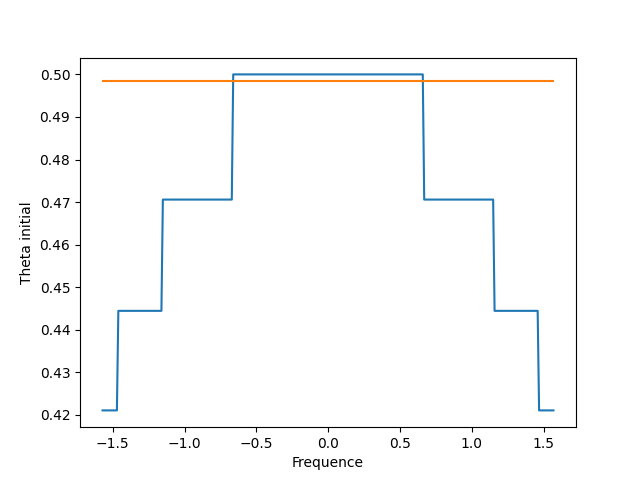
\includegraphics[scale=0.55]{methode.png}
    \caption{Méthode 1}
    \label{fig:methode1}
\end{figure}     
    

La courbe verte sur la figure \ref{fig:methode1} représente la constante $\frac{1}{2\pi}\sqrt(\frac{g}{l})$, car les angles sont en radians. Or, quand $\theta$ est petit, \eqref{eqpendulesimple} devient :
\begin{equation}
    \Ddot{\theta} + \frac{g}{l}\theta = 0
    \label{eqpendulesimplepetitangle}
\end{equation}

Le résultat donné par la figure  est satisfaisant car \eqref{eqpendulesimplepetitangle}, étant de la forme de l'équation d'un oscillateur harmonique, on sait que $f = \frac{1}{2\pi}\sqrt(\frac{g}{l})$. Au voisinage de $0$, il y a presque égalité sur la figure \ref{fig:methode1} entre la constante et la courbe de la fréquence du pendule à un maillon.

\subsection{Pendule à deux maillons}

%On modélise ensuite un pendule à deux maillons, caractérisé par les deux angles $\theta_1$ et $\theta_2$ formés par les deux tiges. 

\subsubsection{Modélisation}

Pour écrire l'équation du mouvement de ce pendule, on a besoin d'exprimer $\Ddot{\theta_1}$ en fonction de $\Dot{\theta_1}$ et de $\theta_1$ et $\Ddot{\theta_2}$ en fonction de $\Dot{\theta_2}$ et de $\theta_2$. Les formules correspondantes sont les suivantes, avec $\omega_1$ la vitesse angulaire du premier maillon, c'est-à-dire $\Dot{\theta_1}$, et $\omega_2$ la vitesse angulaire du deuxième, c'est-à-dire $\Dot{\theta_2}.$ On note $m_i$ et $L_i$ respectivement la masse du ième maillon et la longueur de la ième tige. \\ \\ \\
\begin{equation}
    \Dot{\omega_1}=\frac{-g(2m_1+m_2)\text{sin}\theta_1-m_2g\text{sin}(\theta_1-2\theta_2)-2\text{sin}(\theta_1-\theta_2)m_2(\omega_2^2L_2+\omega_1^2L_1\text{cos}(\theta_1-\theta_2))}{L_1(2m_1+m_2-m_2\text{cos}(2\theta_1-2\theta_2))} 
\end{equation}
\begin{equation}
    \Dot{\omega_2}=\frac{2\text{sin}(\theta_1-\theta_2)(\omega_1^2L_1(m_1+m_2)+g(m_1+m_2)\text{cos}\theta_1+\omega_2^2L_2m_2\text{cos}(\theta_1-\theta_2))}
{L_2(2m_1+m_2-m_2\text{cos}(2\theta_1-2\theta_))}
\end{equation}

\subsubsection{Trajectoire de l'extrémité du pendule}

On souhaite ensuite tracer la trajectoire de l'extrémité du pendule. On résout donc les équations précédentes en utilisant cette fois encore la méthode de Runge-Kutta d’ordre 4, et on trace le résultat sur un graphe.

Afin de montrer la grande dépendance aux conditions initiales de ce système, on trace trois graphes, chacun correspondant à des conditions initiales proches. 

\begin{figure}[!ht]
\minipage{0.32\textwidth}
  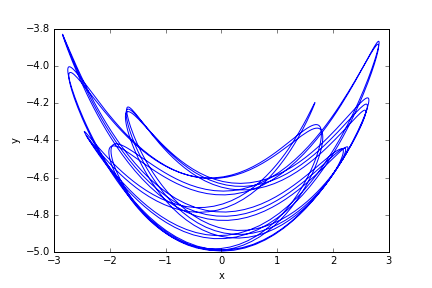
\includegraphics[width=\linewidth]{img1.png}
  \caption{$\theta_1$ = 50°, $\theta_2$ = 70°}
\endminipage\hfill
\minipage{0.32\textwidth}
  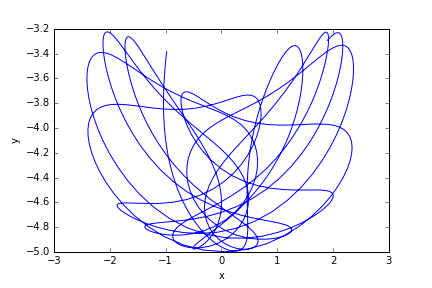
\includegraphics[width=\linewidth]{img3.png}
  \caption{$\theta_1$ = 51°, $\theta_2$ = 70°}
\endminipage\hfill
\minipage{0.32\textwidth}%
  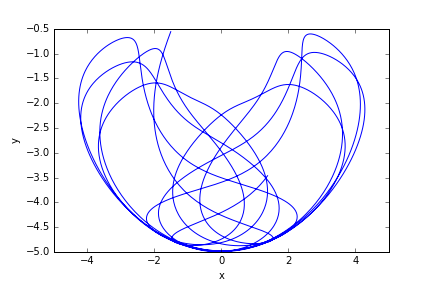
\includegraphics[width=\linewidth]{img2.png}
  \caption{$\theta_1$ = 51°, $\theta_2$ = 71°}
\endminipage
\end{figure}

Ces trois graphes montrent qu'en augmentant un seul des deux angles initiaux d'un degré, la trajectoire obtenue change grandement. Le système est en effet chaotique : il est très sensible aux variations de conditions initiales.   


\subsubsection{Temps de premier retournement}

Le but de cette partie est de représenter le temps de premier retournement d'un pendule à deux maillons, c'est-à-dire le temps au bout duquel les deux maillons du pendule se retrouvent au-dessus du centre du point de son point d'accroche, en fonction des angles initiaux $\theta_1$ et $\theta_2$. Pour déterminer ce temps, nous avons implémenté la fonction $temps\_retournement$, qui le retourne. Cette fonction prend en argument le tableau des valeurs de $\theta_1$, $\Dot{\theta_1}$, $\theta_2$ et $\Dot{\theta_2}$ donné par la méthode de Runge-Kutta d’ordre 4. 

Ensuite, nous avons implémenté la fonction $affiche\_temps\_retournement$. Cette fonction appelle $temps\_retournement$ pour des valeurs de $\theta_1$ et $\theta_2$ qui varient et affiche la matrice des temps de retournements en fonction des valeurs initiales des angles. Cette carte est donnée à la figure \ref{fig:retournement}.

\begin{figure}[ht!]
    \centering
    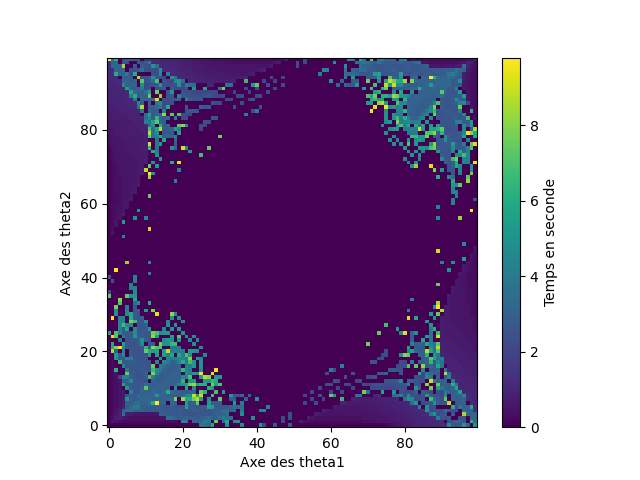
\includegraphics[width=0.5\linewidth]{temps.png}
    \caption{Carte du temps du premier retournement en fonction de $\theta_1$ et $\theta_2$}
    \label{fig:retournement}
\end{figure}



\section{Système proie-prédateur de Lotka-Volterra}
\subsection{Modèle de Malthus}
Le modèle de Malthus est l'un des premiers modèles proposés pour prédire l'évolution d'une ou plusieurs espèces dans un milieu naturel. En considérant une fonction N telle que N(t) représente une population à l'instant t, ce modèle est régi par l'équation différentielle suivante:
\begin{equation}
    \frac{dN(t)}{dt} = bN(t)-dN(t) = \gamma N(t), \quad b,d > 0
\end{equation}
L'équation différentielle fait intervenir deux constantes auxquelles nous pouvons associer une interprétation. En effet, d représente un taux de mortalité par unité de temps et b représente un taux de natalité par unité de temps. La différence des deux constantes: $b-d$ produit une constante gamma. Celle-ci représente une variation de la population. 
\subsection{Modèle de Verhulst}
En réponse au modèle proposé par Malthus qui fait croître une population de manière exponentielle, Verhulst propose un modèle plus précis. En effet, ce modèle prend en compte le fait que plus une population est grande, plus son taux de mortalité est élevé et plus son taux de natalité est faible.
La construction de ce modèle repose sur l'équation différentielle suivante:

\begin{equation}
   \frac{dN(t)}{dt} = \displaystyle\gamma N(t)     \left( 1 - \frac{N(t)}{\kappa} \right),    \quad \gamma, \kappa > 0
\end{equation}
\subsubsection{Résultats graphiques}
Les figures  \ref{fig:malthus} et \ref{fig:verhulst} sont des solutions graphiques au problème pour une population de 1000 personnes sur une période de 3 années.
\begin{multicols}{2}

\begin{figure}[H]
\captionsetup{justification=centering}
      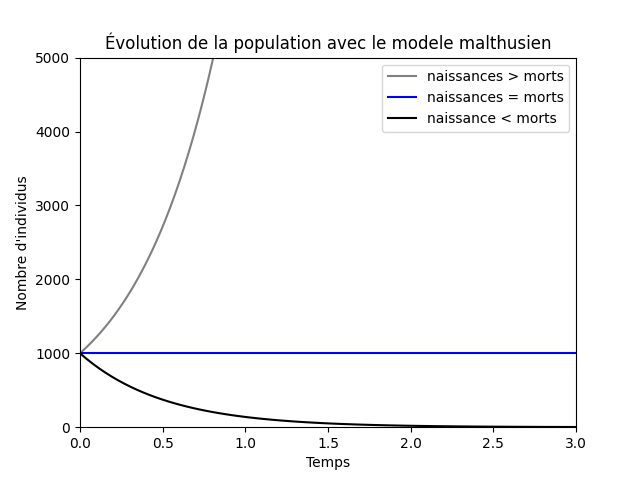
\includegraphics[scale=0.5]{malthusien.png}
      \caption{Modèle de Malthus}
      \label{fig:malthus}
 \end{figure}     
    
    \columnbreak

\begin{figure}[H]
\captionsetup{justification=centering}
      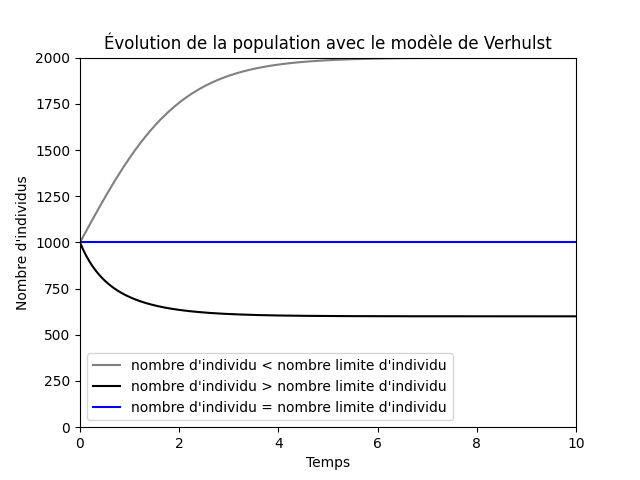
\includegraphics[scale=0.5]{verhulst.png}
      \caption{Modèle de Verhulst}
      \label{fig:verhulst}
\end{figure}

\end{multicols}

Comme attendu, le modèle de Malthus mène la population à une croissance exponentielle. En revanche, le modèle de Verhulst tend à limiter cette divergence.
\subsection{Modèle de Lotka-Volterra}
Les deux premiers modèles, conçus pour les groupes humains, étudient l'évolution d'une population sans prendre en compte les interactions entre ses différentes entités. Le modèle de Lotka-Volterra permet de décrire les interactions entre une population de proies N et une population de prédateurs P. Ce modèle est régi par le système d'équations différentielles suivant:
\begin{equation}
\displaystyle\begin{cases}    \dfrac{dN(t)}{dt} = N(t) (a-bP(t)) \\[3mm]
\dfrac{dP(t)}{dt} = P(t) (cN(t)-d) \\    \end{cases} \quad a, b, c, d > 0
\end{equation}
Afin de mieux comprendre l'origine de ce système, nous allons interpréter les différentes constantes qui interviennent dans celui-ci:

\begin{itemize}
    \item $a$ est le taux de natalité de la population de proies par unité de temps.
    \item $b$ est le taux de mortalité de la population de proies par prédateur et par unité de temps.
    \item $c$ est le taux de natalité de la population de prédateurs par unité de temps et par proie.
    \item $d$ est le taux de mortalité de la population de prédateurs par unité de temps.
\end{itemize}


\newpage
\subsubsection{Résultats graphiques}
\begin{multicols}{2}

\begin{figure}[H]
\captionsetup{justification=centering}
      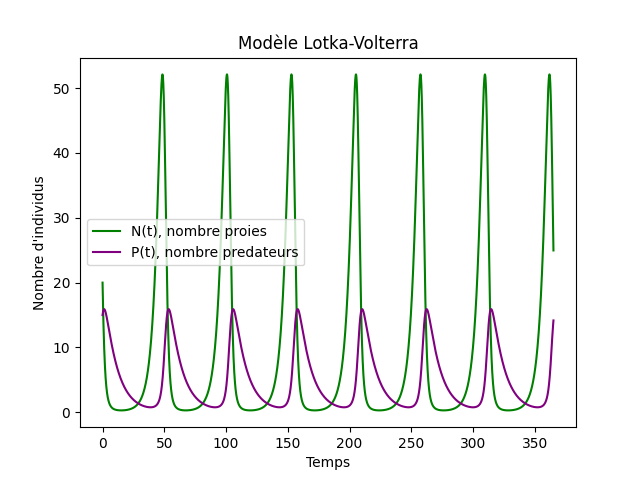
\includegraphics[scale=0.5]{lotka_volterra.png}
      \caption{Variations du couple proies/prédateurs}
      \label{fig:lotka_periodique}
\end{figure}

\columnbreak

 \begin{figure}[H]     
 \captionsetup{justification=centering}
      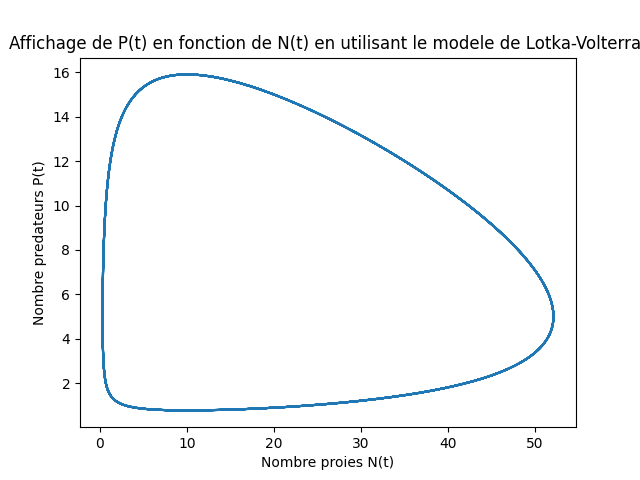
\includegraphics[scale=0.5]{P_N.png}
      \caption{P(t) en fonction de N(t) avec le modèle Lotka-Volterra}
      \label{fig:lotka}
\end{figure}

\end{multicols}
D'une part, nous pouvons constater que si les proies se reproduisent indépendamment des prédateurs, ces derniers influent naturellement sur leur taux de mortalité. D'autre part, le taux de reproduction des prédateurs dépend à l'inverse du nombre de proies qu'ils rencontrent, et leur taux de mortalité est indépendant de la population des proies. Ce cycle engendre deux fonctions périodiques comme le montrent les figures \ref{fig:lotka_periodique} et \ref{fig:lotka}.
\begin{figure}[ht!]
    \centering
    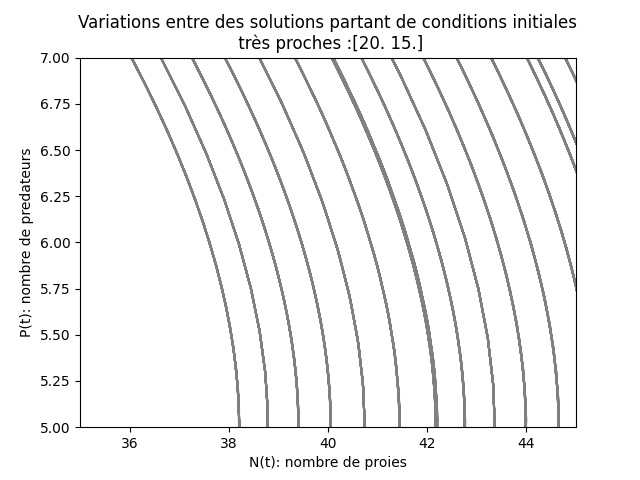
\includegraphics[width=0.5\linewidth]{variations.png}
    \caption{ Variation entre les solutions partant de conditions initiales très proches $\theta_1$ et $\theta_2$}
    \label{fig:solutions}
\end{figure}


Il est remarquable dans la figure \ref{fig:solutions} que lorsque nous agrandissons la différence entre les solutions, les lignes de champ ont une certaine direction. Celles-ci varient selon les points choisis et en particulier pour les points singuliers.

\end{document}
